\chapter{Релейная логика}

\section{Электромагнитное реле}

В конструкторе используются электромагнитные реле с четырьмя
переключающими контактами. В электрических схемах
мы используем нестандартное, но наглядное обозначение таких реле:

\begin{center}
\includegraphics{schemes/one_relay.png}
\end{center}


Контакты $13$ и $14$ подключены к катушке, управляющей состоянием контактов.
Когда напряжение на катушку не подано (и ток через неё не течёт),
контакты переключателей соединены так: $9-1$, $10-2$, $11-3$, $12-4$.

Если же реле включится, подвижная часть контактов сдвинется, разомкнув цепи,
описанные выше, и замкнув следующие: $9-5$, $10-6$, $11-7$, $12-8$.

В каждое реле конструктора встроен светодиод, поэтому можно легко увидеть,
когда оно включается. Это помогает отлаживать схемы или наблюдать
хранящиеся в релейной памяти значения.

Во всех модулях параллельно каждой из катушек реле подключён диод в обратном
направлении. Это сделано для предотвращения искрения контактов других реле
при их размыкании.
Искрение возникает из-за того, что несмотря на разрыв цепи из-за индуктивности катушки
ток должен продолжать течь какое-то время. Но из-за разрыва это невозможно
в обычном режиме, поэтому возникает электрическая дуга, постепенно разрушающая контакты.

\begin{center}
\includegraphics{schemes/diode.png}
\end{center}

Чтобы контакты меньше портились и нужен диод. Оставшийся электрический импульс проходит
уже через него, а не через разомкнутые контакты.

\section{Логические уровни}

При использовании электромагнитных реле логической единице соответствует
наличие напряжения (цепь замкнута), а логическому нулю --- отсутствие напряжения
(цепь разомкнута).

\section{Тумблеры}

\begin{center}
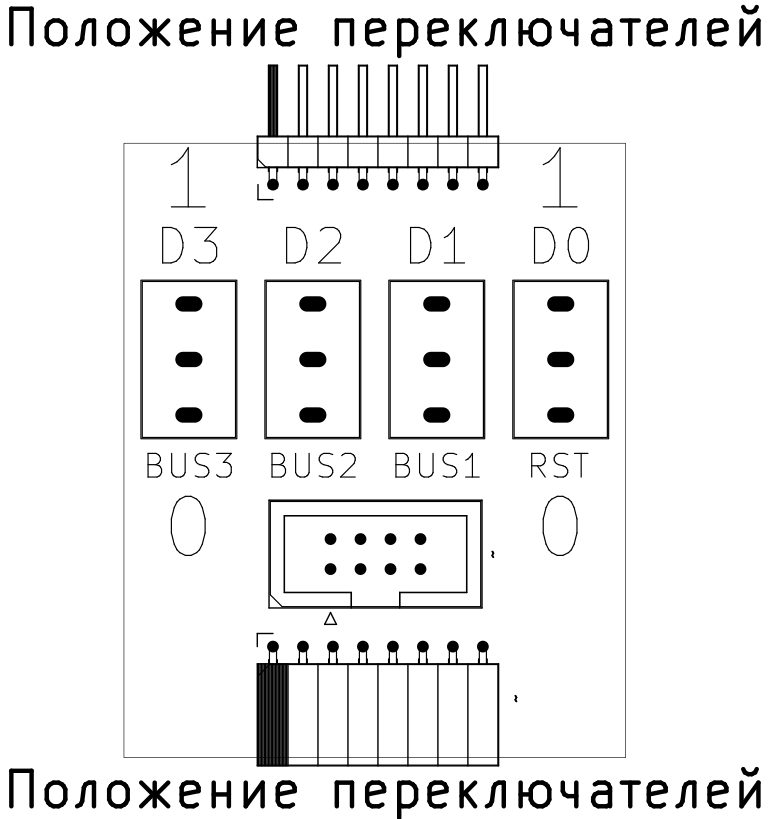
\includegraphics{boards/switches.png}
\end{center}

Модуль с тумблерами используется для ручного включения и выключения реле.
Присоединяя его к разным разъёмам, можно задавать четырёхбитное число,
либо переключать до четырёх управляющих сигналов.

Проще всего проверить работу тумблеров, подключив их к управляющей шине
регистрового модуля, в который вставлены только $4$ реле.

\subsection{Практикум}

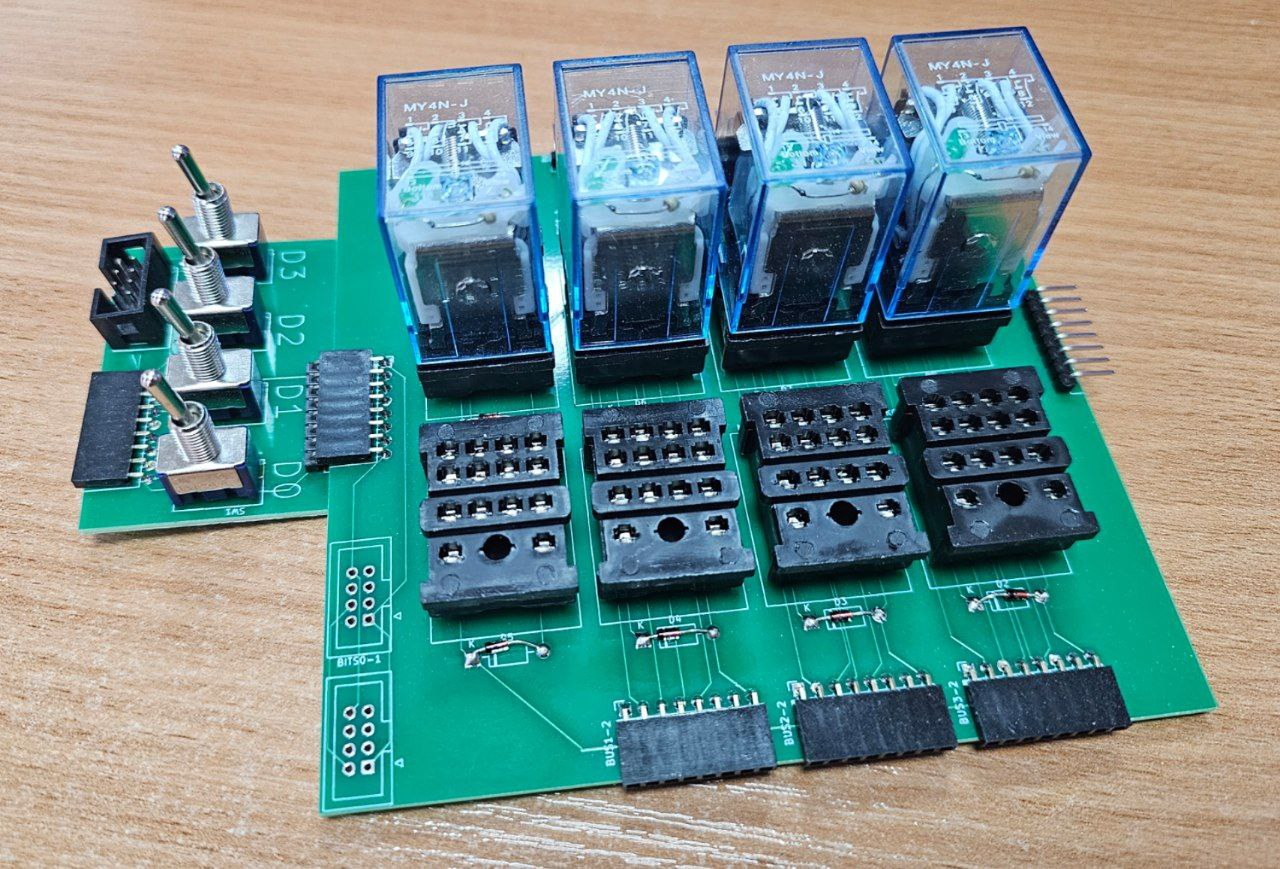
\includegraphics[width=0.5\columnwidth]{photo/switches.jpg}

\begin{enumerate}
    \item Переключать тумблеры. Убедиться, что положение одного тумблера меняет состояние одного реле.
    \item Запомнить включенное и выключенное состояния тумблера, чтобы позднее не было проблем с управлением другими схемами.
\end{enumerate}

\subsection{Задачи}

\begin{enumerate}
    \item Придумать, как соединить тумблеры для выполнения логического ИЛИ.
    \item Придумать, как соединить тумблеры для выполнения логического И.
\end{enumerate}
